\subsection{Supplementary Services}

As the other branches of the prototyping were happening, the need for additional services and infrastructure arose to 
support the development of the prototype as well as to increase the general usability of the prototype. 
This section will especially describe the services which helped to make this prototype a more complete solution.


\begin{figure}[htb]
    \centering
    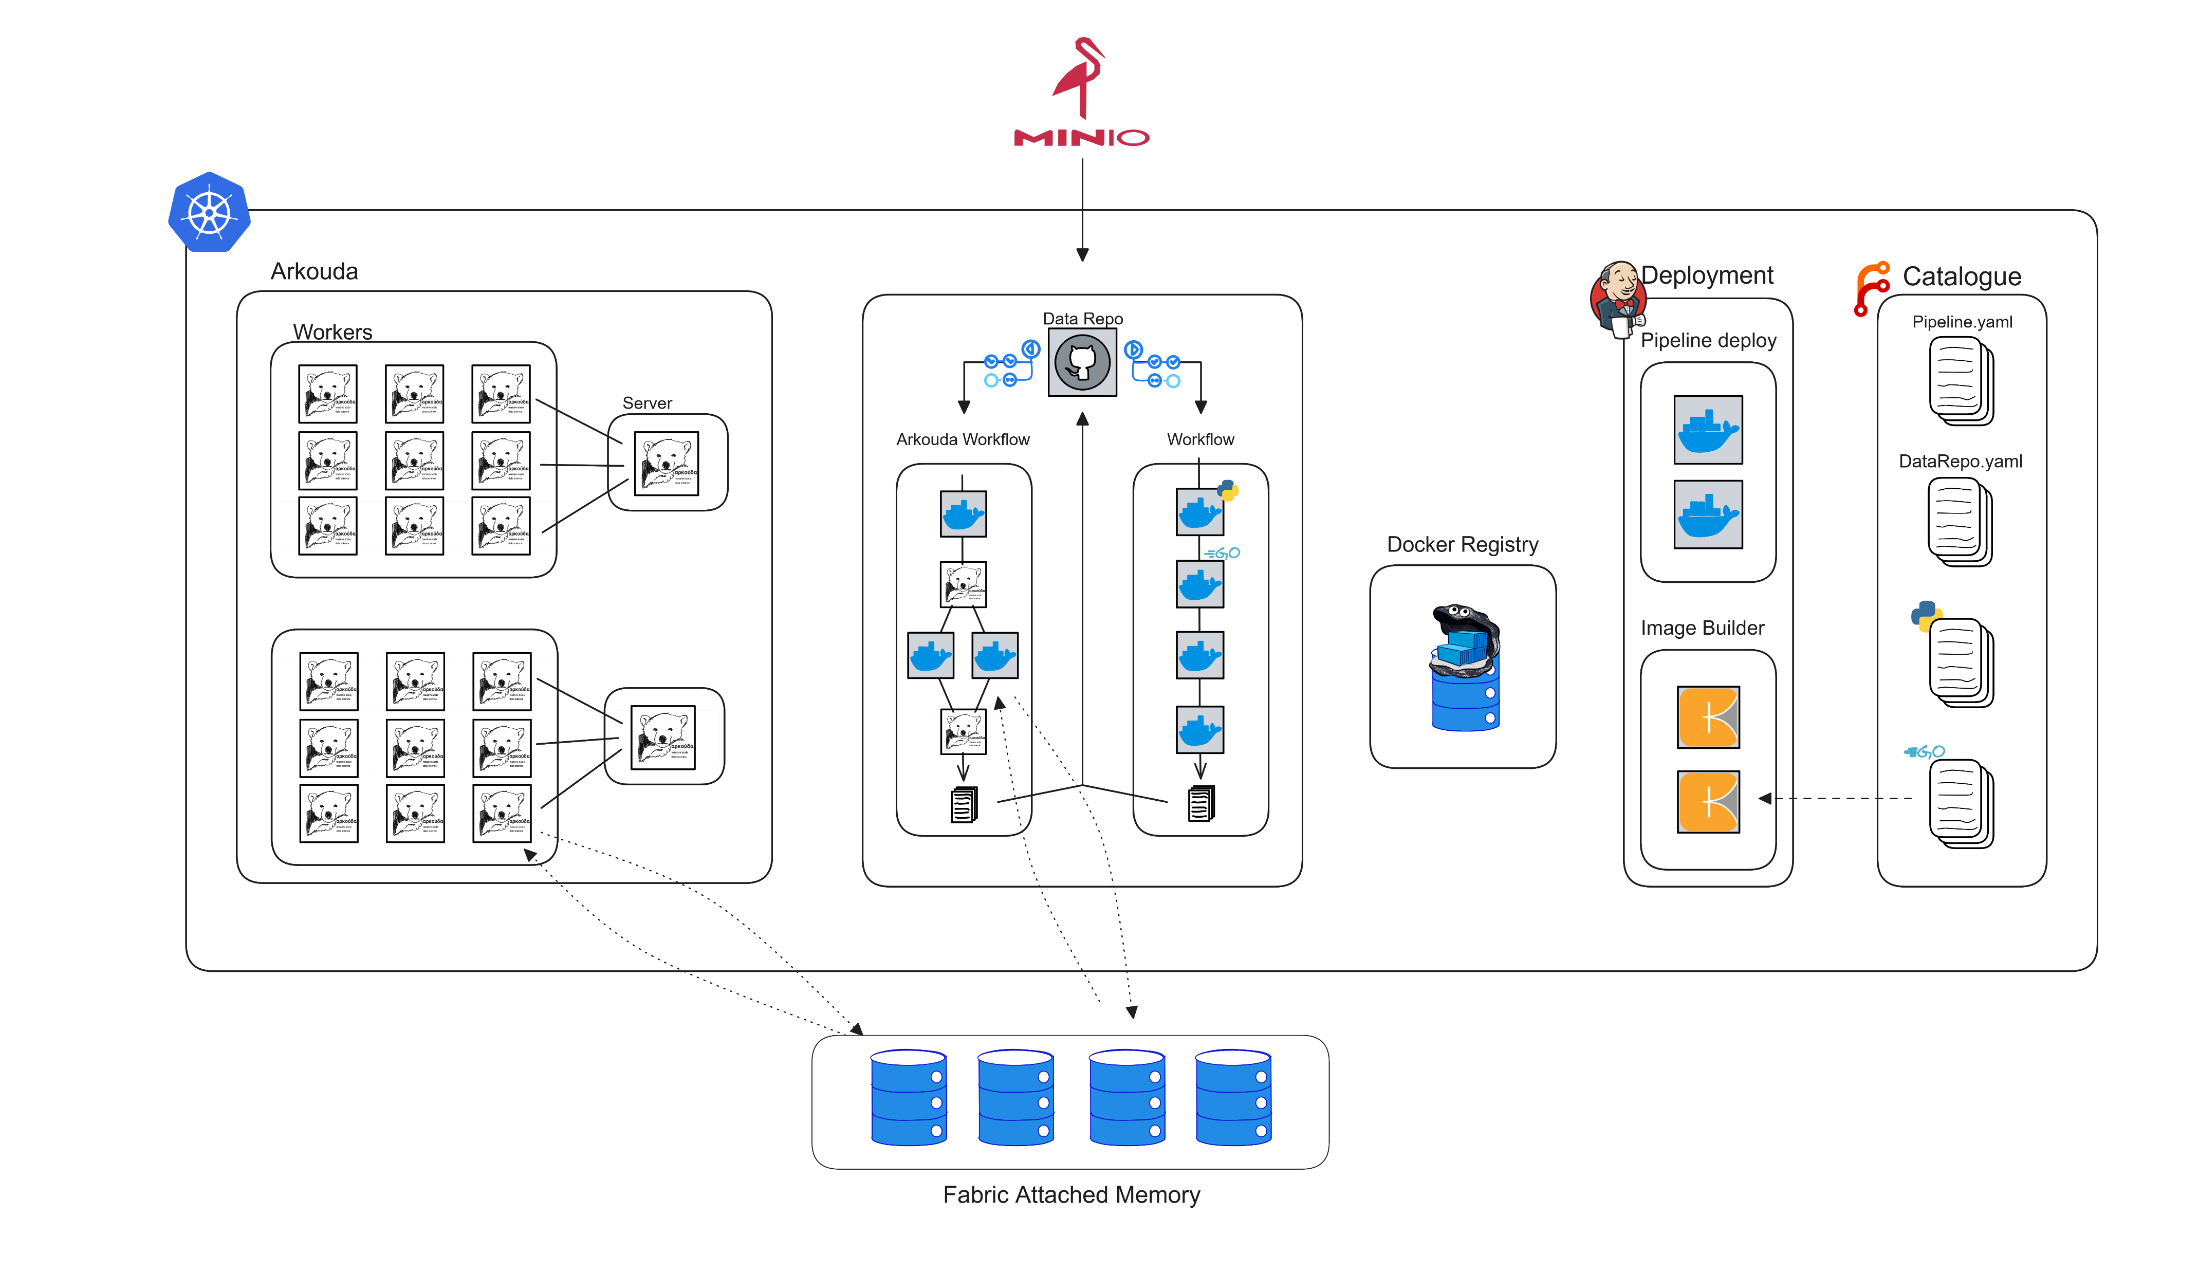
\includegraphics[width=17cm]{graphics/pachykouda_complete.png}
    \caption[Pachyderm High-Level Architecture]{Pachyderm High-Level Architecture}
    \label{abb:pachyderm_complete}
\end{figure}

\subsubsection{Docker Registry}

One thing that was quite apparent from the get go was the need for a central docker registry.
As Pachyderm does not manage the docker images itself, but relies on the user to provide them somehow externally.

During the first iterations when the development was being done on Minikube as described in \ref{minikube}, the internal registry 
of the node was enough.
But as soon as we moved over to the Heydar system keeping the Hosts internal registries in sync was of course not feasible,
Therefore we added a private docker registry to the cluster \footcite{kumarHowSetupPrivate2020}.
The deployment config is based on the official docker registry helm chart\footcite{Dockerregistry10Phntom} and can be found in the projects repo \footcite{eckerthProjectRepoDocker} .

\subsubsection{Forgejo Catalogue}

As this should be the \ac{PoC} of an end user tool, we should also look into usability features and based on previous experience of the team,
the need for a catalogue of previously developed pipelines and processing code was identified.
The idea was to create something similar to the \ac{CLASP} catalogue\footcite{sayersCLoudApplicationServices2015} but for the Pachyderm ecosystem.
This means that users can share, search and deploy workflows from a central catalog, without having to worry about the underlying infrastructure.

Having \ac{HPC} software in a completely contained and versioned system directly addresses many of the original problem statements,
described in \ref{ProblemStatement}, especially the problem of reproducibility, environment management, and the lack of portability.

To start off we, installed a simple github-like interface for the catalogue, called Forgejo\footcite{forgejoForgejo}, which is a fork of the \ac{FOSS} project Gitea\footcite{GiteaGitCup2023},
being maintained by the \ac{NPO} Codeberg e.V.\footcite{codebergCodebergOrg}.
The installation was done using their official helm chart\footcite{Forgejo13Forgejo} and can be found at in the project repo\footcite{eckerthProjectRepoForgejo}.

\subsubsection{Jenkins}

Now that we have a place to hold and version the code files and a place to hold the resulting docker images, we need a way to build and deploy them automatically.
For that purpose an installation of Jenkins was added to the Cluster. Jenkins is a \ac{FOSS} \ac{CI/CD} tool, which is widely used in industry \footcite{JenkinsMarketShare}.
It enables us to execute arbitrary code in an controlled environment based on triggers or schedules.
We will be using it to automatically build and deploy docker images whenever code is pushed to the Forgejo catalogue, as well as automatically deploying pipeline scripts to Pachyderm.

By using this we ensure that the code and the docker images are always in sync and that the user does not have to worry about building and deploying the images manually or interacting with the underlying Cluster.
We also extend the factor of provenance which was limited to the data itself, to the containers code and pipeline spec as well, now having total oversight into which input begets what output.
This was achieved in multiple steps as this turned out to be quite an involved process.

First off was of course the general installation of the project into the cluster based on the image provided by Jenkins \footcite{JenkinsJenkinsJenkinsci}.
Then we have to integrate Jenkins into the the Kubernetes cluster as well, as we want it to be able to spawn its own worker pods within the cluster to handle the building of the containers and pushing of the pipelines.
Also an integration with the Forgejo catalogue was needed, so that Jenkins would be informed about new commits to the catalogue and could start the building process.

The installation instructions, \ac{RBAC} and the configuration of the Jenkins installation can be found at \ref{appendix:cicd_installation_instructions}.

\subsubsection{CI/CD Pipeline}

Now that we have a Jenkins installation which is able to spawn its own worker pods on the cluster and have set up system wide Webhooks for the Forgejo catalogue,
which will inform Jenkins about every new commit to any repository on the catalogue, we will need to develop a pipeline which will tell Jenkins what to do if a new commit is detected.

As the Pachyderm team say themselves, "\textit{[...] users with limited experience with containerization, cloud computing, and distributed systems may find it challenging to use Pachyderm effectively.}" \footcite{PachydermTargetAudience2023}
Unfortunate many \acp{SME} are more focused on their domain specific knowledge and usually only have a limited understanding of the underlying infrastructure, an effect which has already been noticed in classical \ac{HPC} \footcite{shenoiHPCEducationDomain2019}, 
which is likely more pronounced in a field which has only recently started to gain traction in the wider scientific community.

Therefore providing an way to deploy code and pipelines while minimizing the interaction with the underlying infrastructure is a key feature of this part of the prototype.
The goal is to create a pipeline which can take a regular software project form the Forgejo catalogue, make reasonable assumptions about the project structure and build the required docker images and deploy the pipeline to Pachyderm.

A completely functional Pachyderm project, consisting of a $N$ processing steps requires the following components:

\begin{itemize}
    \item $N$ code files, one for each processing step
    \item $N$ Dockerfiles, one for each processing step
    \item $N$ pipeline specifications, one for each processing step
    \item At least one description file for the data repository(s)
    \item If needed supporting files, which should be included in one ore more image, but should not get their own.
\end{itemize}

However as we want to minimize the interaction with the underlying infrastructure, we want to minimize the amount of input the user has to provide, without restricting the knowing users.
In order to achieve this, the pipeline first detects the existence of the above components.
We then try to make a reasonable assumption about the structure of the project and the relation between the components, considering: directory structure, naming conventions, and static code analysis.
The pipeline will then try to fill in gaps in the project structure, like missing Dockerfile by using default values and insights gained form the previous steps.
The pipeline itself is written in a mix of Groovy, Python and bash, a flowchart describing the process in more detail can be found in the appendix at \ref{abb:flowchart_pipeline_upper} its code can be found in the projects repo\footcite{eckerthProjectRepoJenkins}.

There was also a custom container image created, extending official Jenkins worker image\footcite{JenkinsJenkinsDocker}, enabling us to build docker images from within a running container in the cluster by using a dedicated kaniko 
sidecar container \footcite{KanikoBuildImages2023} which enables us to build docker images without having to run Docker in Docker, which is not recommended \footcite{UsingDockerinDockerYour}.
The image also contains the necessary tools to interact with the Pahcyderm API and to run the Python scripts which are used to analyze the project structure and do t   e code generation, it can be found in the project Repo\footcite{eckerthProjectRepoJenkinsa}.

While this pipeline does technically work, it is still still quite finicky and is missing many edgcases and does need further development to be able to handle more thant the most basic projects.
Even though its development was cut short it does show the potential of this approach and how it could be used to make the Pachyderm ecosystem more accessible to users which are not as familiar with the underlying infrastructure, 
while still allowing more experienced users to interact with the system directly.